% !TeX TS-program = xelatex

\documentclass[11pt, a4paper]{report}

% Dokumentum adatok
% =================
\author{}
\title{Műszaki áramlástan feladatgyűjtemény}

% A közös fájlok beszúrása
% ========================
\newcommand*{\JakiFolder}{./JAKI}%

% A közös fájlok a JAKI tárolóban vannak, amit az MHFGY-vel 
% közös mappába kell letölteni (clone/pull).

% A "book" dokumentumosztály fölösleges oldalakat szúr be a címoldal
% és a tartalomjegyzék után.

\usepackage[utf8]{inputenc}
\usepackage[magyar]{babel}

% XeLaTeX ékezetes betűk
\usepackage{fontspec}

% A margók beállítása, később a 
%	\newgeometry{left=3cm,bottom=0.1cm}
% és a 
%	\restoregeometry
% parancsokkal egyedileg módosíthatók a margók
\usepackage[left=2cm, right=2cm, top=2cm, bottom=2cm]{geometry}

\usepackage{amsmath}
\usepackage{amssymb}

% A dupla betűk betűtípusának beállítása
\AtBeginDocument{
	\DeclareSymbolFont{AMSb}{U}{msb}{m}{n}
	\DeclareSymbolFontAlphabet{\mathbb}{AMSb}
}

% A régi német betűtípusok támogatása (fraktúra, Schwabacher, gót)
% A gót betűtípus nem működik
% Az ékezetes betűk csak a Table 18: Text-mode Accents táblázat szerint működnek
\usepackage{yfonts}

% Tabu hiba kezelés
\usepackage{booktabs}% http://ctan.org/pkg/booktabs
\newcommand\tabitem{\makebox[1em][r]{\textbullet~}}
\usepackage{tabto}
\usepackage{tabu}

% Bekeretezett részek
\usepackage[framemethod=tikz]{mdframed}
% Megjegyzés
\newcommand{\comment}[2][black!10]{%
\begin{mdframed}[hidealllines=true, backgroundcolor=#1, innerleftmargin=3pt, innerrightmargin=3pt, leftmargin=-3pt, rightmargin=-3pt]
Megjegyzés: #2
\end{mdframed}
}

%\usepackage{titlesec}

\pagestyle{plain}

\usepackage{float}
\usepackage{xifthen}

% Tizedesvessző
\usepackage{icomma}

% Függelék

\usepackage[toc,titletoc,page]{appendix}
\renewcommand{\appendixtocname}{Függelékek}
\renewcommand{\appendixpagename}{Függelékek}


%\fontspec{Times New Roman}
%\setmonofont{Consolas}
%\setmainfont{Calibri}

\usepackage{commath}
% A \Dif esetén a hatványkitevők rálógnak a D-re.
% A deriváltakban a d után sok az üres hely.

% This package will provide a complete implementation of 
% unicode maths for XELATEX and LuaLATEX.
% A Cambria Math támogatott.
% Javítja a vektor jelek elhelyezését a betűk felett.
% Az alsó és felső indexek betűtípusait módosítja, és szélesebbek a betűk.
\usepackage[math-style=TeX]{unicode-math}
%\setmathfont{XITS Math} % Túl vastagok a betűk
%\setmathfont{Cambria Math}

\usepackage{siunitx}
\sisetup{
	per-mode = fraction,
	fraction-function = \dfrac,
	detect-family = true,
	output-decimal-marker = {,},
	space-before-unit = true,
	use-xspace = true,
	exponent-product = \cdot,
	sticky-per = true
}

\usepackage[makeroom]{cancel}

% Többrészes ábrák létrehozása, subfigure környezet
\usepackage[justification=centering]{caption}
\usepackage{subcaption}

% A Hyperref csomagot lehetőleg utolsóként kell betölteni.
\usepackage[colorlinks=false]{hyperref}

% A címsorok másolása a kereszthivatkozásokba
\usepackage{nameref}

% Bekarikázott számok
\usepackage{pifont}

% Kiemelés színnel
\usepackage{xcolor}

% Az oszlopvektorok és mátrixok jelölésére
\usepackage{accents}
\newcommand{\ubar}[1]{\underaccent{\bar}{#1}}

% Színes táblázat, a tabuhoz nem szükséges
%\usepackage{colortbl}

% Fekvő oldalak
% If you are using pdfLaTeX, you should use pdflscape instead. The pdflscape package adds PDF support to the landscape environment of package lscape, by setting the PDF/Rotate page attribute. Pages with this attribute will be displayed in landscape orientation by conforming PDF viewers:
\usepackage{pdflscape}

% Kiemelés
% Több sorba osztásnál %-ezni kell a sortöréseket
%\newcommand{\highlight}[2]{\colorbox{#1}{$\displaystyle#2$}}

% Függőleges távolságok
\newcommand{\reducedstrut}{\vrule width 0pt height 1.2\ht\strutbox depth 0.95\dp\strutbox\relax}
\newcommand{\highlight}[2]{%
  \begingroup
  \setlength{\fboxsep}{1pt}% Vízszintes távolság
  \colorbox{#1}{\reducedstrut$\displaystyle#2$\/}%
  \endgroup
}

% Sortáv módosítás
\usepackage{setspace}
%\singlespacing
%\onehalfspacing
%\doublespacing

% Felsorolások
\usepackage{enumitem}

% Megjegyzés létrehozás
%\newlist{notes}{enumerate}{1}
%\setlist[notes]{label=Megjegyzés: , leftmargin=*}

% Külső fájlok írása
% Elvileg szükségtelen
%\usepackage{filecontents}

% Forráskezelés
%When using babel or polyglossia with biblatex, loading csquotes is recommended to ensure that quoted texts are typeset according to the rules of your main language.
\usepackage{csquotes}
\usepackage[ 
	backend=biber, 
	url=false, 
	citestyle=numeric,%draft,
	bibstyle=numeric,%style=numeric,%authoryear,%numeric, 
	giveninits=true, 
	clearlang=true, 
	bibencoding=auto,
	sorting=none]{biblatex}
	
\makeatletter

\newrobustcmd*{\parentexttrack}[1]{%
  \begingroup
  \blx@blxinit
  \blx@setsfcodes
  \blx@bibopenparen#1\blx@bibcloseparen
  \endgroup}

\AtEveryCite{%
  \let\parentext=\parentexttrack%
  \let\bibopenparen=\bibopenbracket%
  \let\bibcloseparen=\bibclosebracket}

\makeatother


% Az egyenletek előtti és utáni térközök beállítása
% A TikZ blokkdiagamban a 3. szinttől lefele fölösleges bal margót hoz létre (???)
%
% => NE LEGYEN ÜRES SOR AZ EGYENLETEK ELŐTT!
%
%\makeatletter
%\g@addto@macro\normalsize{%
%	\setlength\abovedisplayskip{6pt}
%	\setlength\belowdisplayskip{12pt}
%	\setlength\abovedisplayshortskip{0pt}
%	\setlength\belowdisplayshortskip{12pt}
%}
%\makeatother

% Az árva- és özvegysorok büntetése (nem biztos, hogy nem lesznek...)
\widowpenalty10000
\clubpenalty10000


% SAJÁT PARANCSOK LÉTREHOZÁSA
% ===========================

\DeclareMathOperator{\tr}{tr}

% Gradiens, forráserősség, örvényerősség
\newcommand{\Grad}[1] {\mathrm{grad\,} #1}
\newcommand{\Div}[1] {\mathrm{div\,} #1}
\newcommand{\Rot}[1] {\mathrm{rot\,} #1}
\newcommand{\Diag}[1] {\mathrm{diag\,} #1}

% Függvények
\newcommand{\Det}[1] {\mathrm{det} #1}
\DeclareMathOperator{\tg}{tg}
\DeclareMathOperator{\sgn}{sgn}
\DeclareMathOperator{\arctg}{arctg}
\DeclareMathOperator{\arctgNN}{arctg2}

% Mátrix belső közei
\makeatletter
\renewcommand*\env@matrix[1][\arraystretch]{%
	\edef\arraystretch{#1}%
	\hskip -\arraycolsep
	\let\@ifnextchar\new@ifnextchar
	\array{*\c@MaxMatrixCols c}}
\makeatother

% Oszlopvektor, sorvektor és mátrix jelölések
\newcommand{\mat}[1] {\underline{\underline{#1}}\reducedstrut}
\newcommand{\cvec}[1] {\underline{#1}\reducedstrut}
%\def\rvec#1{\underline{#1}^{T}}
%\def\mat#1{\underline{\underline{#1}}}
%\def\mat3#1{\underline{\underline{\underline{#1}}}}

\newcommand{\vektor}[2][1]{\begin{bmatrix}[#1] #2 \end{bmatrix}}
\newcommand{\tmb}[2][2]{\begin{bmatrix}[#1] #2 \end{bmatrix}}
\newcommand{\vek}[4][1]{\begin{bmatrix}[#1] #2 \\ #3 \\ #4 \end{bmatrix}}
\newcommand{\mtrx}[1]{\begin{bmatrix}#1\end{bmatrix}}



% FÜGGELÉK TARTALOMJEGYZÉK
% Appendix csomag (appendix.sty)
%\newcommand{\@redotocentry@pp}[1]{%
%  \let\oldacl@pp=\addcontentsline
%  \def\addcontentsline##1##2##3{%
%    \def\@pptempa{##1}\def\@pptempb{toc}%
%    \ifx\@pptempa\@pptempb
%      \def\@pptempa{##2}\def\@pptempb{#1}%
%      \ifx\@pptempa\@pptempb
%\oldacl@pp{##1}{##2}{##3}%A kísérleti változat: \oldacl@pp{##1}{##2}{\appendixname\space [##1][##2][##3] (\@car \splitlist{##3}\@nil) (\@cdr \splitlist{##3}\@nil)}%
%      \else
%        \oldacl@pp{##1}{##2}{##3}%
%      \fi
%    \else
%      \oldacl@pp{##1}{##2}{##3}%
%    \fi}
%}


% VÁLTOZÓK
\makeatletter
\let\JakiTitle\@title
\let\JakiAuthor\@author
\makeatother

% OLDALSZÁMOZÁS
% Oldalszámozás váltás a kezdő, a fő és a befejező szakasz határán
% A "report" osztályban nincs, a "book" osztályból másolva...
%https://tex.stackexchange.com/questions/154646/is-there-an-easy-way-to-get-the-frontmatter-mainmatter-and-backmatter-in-a-l
\makeatletter
\newcommand\frontmatterreport{%
	\cleardoublepage
	%\@mainmatterfalse
	\pagenumbering{Roman}}

\newcommand\mainmatterreport{%
	\cleardoublepage
	%\@mainmattertrue
	\pagenumbering{arabic}}

\newcommand\backmatterreport{%
	\if@openright
		\cleardoublepage
	\else
		\clearpage
	\fi
	% \@mainmatterfalse
	}
\makeatother


% HYPERREF
\hypersetup{
	pdftitle={\JakiTitle}, 
	pdfauthor={\JakiAuthor}, 
	colorlinks = true,
	citecolor = orange,
	filecolor = red,
	linkcolor = blue,
	urlcolor = red
}


% Az átmérőjel alapvonalra emelése
%\makeatletter
%\let\olddiameter\diameter
%\renewcommand{\diameter}[0]{\raisebox{\depth}{\olddiameter}}
%\makeatother

				% Formázás, csomagok

% TikZ - Ábrázolás
% ================
\usepackage{tikz} 
\usepackage{tikz-3dplot}
\usetikzlibrary{arrows.meta, automata, bending, calc, decorations.markings, fit, graphs, intersections, patterns, positioning, scopes, shapes, shapes.geometric, shapes.multipart, trees}
% bending: a nyílfejek "elnyomják" az íveket, ez a könyvtár helyre teszi...

\usepackage{pgfplots}
\pgfplotsset{compat=1.10}
\usepgfplotslibrary{fillbetween}

% Szögek méretezése
% =================

\pgfkeys{/tikz/.cd, % to set the path
	xa/.initial=0, % initial value
	xa/.get=\xa, % to get the value from a macro
	xa/.store in=\xa, % to store the value into a macro
	xb/.initial=0,
	xb/.get=\xb,
	xb/.store in=\xb,
	ya/.initial=0,
	ya/.get=\ya,
	ya/.store in=\ya,
	yb/.initial=0,
	yb/.get=\yb,
	yb/.store in=\yb,
	ra/.initial=1.25 cm,
	ra/.get=\ra,
	ra/.store in=\ra,
	rb/.initial=1.5 cm,
	rb/.get=\rb,
	rb/.store in=\rb,
	rm/.initial=0.5cm,			% \pgfangle: sugár a méretvonal töréspontjáig
	rm/.get=\rm,
	rm/.store in=\rm,
	a/.initial=0,				% \pgfangle: szög (honnan); \pgflength: nyílfej van/nincs
	a/.get=\a,
	a/.store in=\a,
	b/.initial=45,				% \pgfangle: szög (hova); \pgflength: nyílfej van/nincs
	b/.get=\b,
	b/.store in=\b,
	lv/.initial=45,
	lv/.get=\lv,
	lv/.store in=\lv,
	lm/.initial=0.5,
	lm/.get=\lm,
	lm/.store in=\lm,
	alim/.initial=0,			% \pgflength: 0/[1] bal és jobb méretsegédvonal
	alim/.get=\alim,
	alim/.store in=\alim,
	blim/.initial=0,
	blim/.get=\blim,
	blim/.store in=\blim,
	ny/.initial=1,				% \pgflength: 0/[1] a méret elforgatása (csak függőleges esetben)
	ny/.get=\ny,				% \pgfangle: nyíl/kör kiosztás
	ny/.store in=\ny,
	szín/.initial=black,
	szín/.get=\szín,
	szín/.store in=\szín,
	belül/.initial=0,		% \pgfangle: 0/1/2/3, \pgflength: 0/[1]/2 a méret helye
	belül/.get=\belül,
	belül/.store in=\belül,
	horgony/.initial=south west,		% \pgfangle, \pgfpont: a méret jelének/pont nevének horgonyzása
	horgony/.get=\horgony,
	horgony/.store in=\horgony,
	ztengely/.store in=\ztengely,
	xsh/.initial=0,
	xsh/.get=\xsh,
	xsh/.store in=\xsh,
	ysh/.initial=0,
	ysh/.get=\ysh,
	ysh/.store in=\ysh
	}

\newcommand{\pgfangle}[2][]{ %
	% Az alapértelmezett értékek visszaállítása
	\tikzset{alim=0, blim=0, szín=black, belül=0, ra=1.25, ny=1, rm=0.5, horgony=south, xsh=0, ysh=0}
	
	\tikzset{#1} % Az első argumentum a tulajdonságlista
	% (\xa, \ya) a szög csúcspontja
	% \ra az ív sugara, \rb a szög szárainak hossza
	
	% PÉLDA: \pgfangle[ra=1.25, a=\alf, b=0, blim=1]{$\alpha$};
	
	\tikzset{rb = \ra + 0.25} % a külső sugár
	\tikzset{lv = {\ra*abs(\b-\a)*3.14159/180}} % az ívhossz
	\tikzset{>={Triangle[length=4mm, width=1.25mm]}} % lokális nyílfej beállítás
	
	% A kezdőpont
	\coordinate (O) at (\xa, \ya);
	
	% A két szár és az ív végpontjai
	\coordinate (A) at ($(O) + (xyz polar cs: radius=\ra, angle=\a)$);
	\coordinate (U) at ($(O) + (xyz polar cs: radius=\rb, angle=\a)$);
	\coordinate (B) at ($(O) + (xyz polar cs: radius=\ra, angle=\b)$);
	\coordinate (V) at ($(O) + (xyz polar cs: radius=\rb, angle=\b)$);
	
	\ifnum\belül=0
		% Jobbra
		\pgfmathsetmacro{\ivalfa}{1.0/\ra*180/3.14159};
		\pgfmathsetmacro{\ivbeta}{0.5/\ra*180/3.14159};
	\else
		\ifnum\belül=2
			% Balra
			\pgfmathsetmacro{\ivalfa}{0.5/\ra*180/3.14159};
			\pgfmathsetmacro{\ivbeta}{1.0/\ra*180/3.14159};
		\else
			% A körcikken belül vagy külső vonalon
			\pgfmathsetmacro{\ivalfa}{0.5/\ra*180/3.14159};
			\pgfmathsetmacro{\ivbeta}{0.5/\ra*180/3.14159};
		\fi
	\fi
	
	\ifnum\ny=0
		% Az ív nyílfejek nélkül
		\draw[name path=iv, \szín] (A) arc [start angle=\a, end angle=\b, radius=\ra];
	\fi
	\ifnum\ny=1
		% Az ív nyílfejekkel
		\pgfmathparse{\lv > 1.0 ? int(1) : int(0)}
		\ifnum\pgfmathresult=1 
			% Belső nyílfejek
			\draw[name path=iv, \szín, <->] (A) arc [start angle=\a, end angle=\b, radius=\ra];
		\else
			% Külső nyílfejek
			\draw[name path=iv, \szín] (A) arc [start angle=\a, end angle=\b, radius=\ra];
			
			\draw[\szín, <-] (A) arc [start angle=\a, end angle={\a-\ivalfa}, radius=\ra];
			\draw[\szín, <-] (B) arc [start angle=\b, end angle={\b+\ivbeta}, radius=\ra];
		\fi
	\fi
	\ifnum\ny=2
		% Az ív nyílfejjel és kezdőkörrel jobboldalon
		\pgfmathparse{or(equal(\belül, 1), equal(\belül, 3))}
		\ifnum\pgfmathresult=1 
			% Belső felirat
			\pgfmathparse{\lv > 1.0 ? int(1) : int(0)}
			\ifnum\pgfmathresult=1 
				% Belső nyílfej
				\draw[name path=iv, \szín, ->] (A) arc [start angle=\a, end angle=\b, radius=\ra];
			\else
				% Külső nyílfej
				\draw[name path=iv, \szín] (A) arc [start angle=\a, end angle=\b, radius=\ra];
				
				\draw[\szín, -] (A) arc [start angle=\a, end angle={\a-\ivalfa}, radius=\ra];
				\draw[\szín, <-] (B) arc [start angle=\b, end angle={\b+\ivbeta}, radius=\ra];
			\fi
		\else
			% Külső felirat (belül = 0 vagy 2)
			\ifnum\belül=2
				% A nyílfej mindig kívül balra
				\draw[name path=iv, \szín] (A) arc [start angle=\a, end angle=\b, radius=\ra];
				\draw[\szín, <-] (B) arc [start angle=\b, end angle={\b+\ivbeta}, radius=\ra];
			\else
				\pgfmathparse{\lv > 1.0 ? int(1) : int(0)}
				\ifnum\pgfmathresult=1 
					% Belső nyílfej)
					\draw[name path=iv, \szín, ->] (A) arc [start angle=\a, end angle=\b, radius=\ra];
				\else
					% Külső nyílfej
					\draw[name path=iv, \szín] (A) arc [start angle=\a, end angle=\b, radius=\ra];
					
					\draw[\szín, -] (A) arc [start angle=\a, end angle={\a-\ivalfa}, radius=\ra];
					\draw[\szín, <-] (B) arc [start angle=\b, end angle={\b+\ivbeta}, radius=\ra];
				\fi
			\fi
		\fi
		
		% A kezdőkör jobboldalon
		\draw[black, fill=white] ({\ra*cos(\a)}, {\ra*sin(\a)}) circle[radius=0.5mm];
	\fi
	\ifnum\ny=3
		% Az ív nyílfejjel és kezdőkörrel baloldalon
		\pgfmathparse{or(equal(\belül, 1), equal(\belül, 3))}
		\ifnum\pgfmathresult=1 
			% Belső felirat
			\pgfmathparse{\lv > 1.0 ? int(1) : int(0)}
			\ifnum\pgfmathresult=1 
				% Belső nyílfej
				\draw[name path=iv, \szín, <-] (A) arc [start angle=\a, end angle=\b, radius=\ra];
			\else
				% Külső nyílfej
				\draw[name path=iv, \szín] (A) arc [start angle=\a, end angle=\b, radius=\ra];
				\draw[\szín, <-] (A) arc [start angle=\a, end angle={\a-\ivalfa}, radius=\ra];
			\fi
			
		\else
			% Külső felirat (belül = 0 vagy 2)
			\ifnum\belül=0
				% A nyílfej mindig kívül jobbra
				\draw[name path=iv, \szín] (A) arc [start angle=\a, end angle=\b, radius=\ra];
				\draw[\szín, <-] (A) arc [start angle=\a, end angle={\a-\ivalfa}, radius=\ra];
			\else
				\pgfmathparse{\lv > 1.0 ? int(1) : int(0)}
				\ifnum\pgfmathresult=1 
					% Belső nyílfej)
					\draw[name path=iv, \szín, <-] (A) arc [start angle=\a, end angle=\b, radius=\ra];
					\draw[\szín, -] (B) arc [start angle=\b, end angle={\b+\ivbeta}, radius=\ra];
				\else
					% Külső nyílfej
					\draw[name path=iv, \szín] (A) arc [start angle=\a, end angle=\b, radius=\ra];
					\draw[\szín, -] (B) arc [start angle=\b, end angle={\b+\ivbeta}, radius=\ra];
					\draw[\szín, <-] (A) arc [start angle=\a, end angle={\a-\ivalfa}, radius=\ra];
				\fi
			\fi
		\fi
		
		% A kezdőkör baloldalon
		\draw[black, fill=white] ({\ra*cos(\b)}, {\ra*sin(\b)}) circle[radius=0.5mm];
	\fi
	
	%\pgfmathparse{\lv}
	%\node[blue](X){\lv = \pgfmathresult};
	
	% Az ív felezőpontja (a "bending" könyvtárral nem kell a metszéspont...)
	%\coordinate (S) at ($(O) + (xyz polar cs: radius=2*\rb, angle={(\a+\b)/2})$);
	%\path[name path=O--S] (O) -- (S);
	%\path[name intersections={of=iv and O--S}];
	%\coordinate (T) at (intersection-1);
	% Másik módszer:
	%\draw[name intersections={of=V and O--S, by=W}][very thick,orange] (1,0) -- (W);
	
	% A méretezés pontjai
	\coordinate (P) at ($(O) + (xyz polar cs: radius=\ra, angle={(\a+\b)/2})$);
	\coordinate (Q) at ($(P) + (xyz polar cs: radius=\rm, angle={(\a+\b)/2})$);
	
	\pgfmathparse{abs(\a+\b)/2 < 90 ? int(1) : int(0)}
	\ifnum\pgfmathresult=1 
		\coordinate (R) at ($(Q) + (xyz polar cs: radius=\lm, angle=0)$);
		\coordinate (S) at ($(Q) + (xyz polar cs: radius=\lm/2, angle=0)$);
	\else
		\coordinate (R) at ($(Q) + (xyz polar cs: radius=-\lm, angle=0)$);
		\coordinate (S) at ($(Q) + (xyz polar cs: radius=-\lm/2, angle=0)$);
	\fi
	
	% A méretvonalak (alim és blim szerint)
	\ifnum\alim=1\draw[black] (O) -- (U);\fi
	\ifnum\blim=1\draw[black] (O) -- (V);\fi
	
	% A méret felirat
	\pgfmathsetmacro{\aha}{0.4/\ra*180/3.14}
	\ifnum\belül=0
		% A körcikken kívül jobbra
		\coordinate (W) at ($(O) + (xyz polar cs: radius={\ra+0.25}, angle={((\a-\aha)+(\a-\ivalfa))/2})$);
		\node[\szín, anchor={\horgony}, xshift={\xsh}, yshift={\ysh}] at (W) {#2};
	\fi
	\ifnum\belül=1
		% A körcikken belül
		\coordinate (W) at ($(O) + (xyz polar cs: radius={\rb-0.5}, angle={(\a+\b)/2})$);
		\node[\szín, anchor=center, xshift={\xsh}, yshift={\ysh}] at (W) {#2};
	\fi
	\ifnum\belül=2
		% A körcikken kívül balra
		\coordinate (W) at ($(O) + (xyz polar cs: radius={\ra+0.25}, angle={((\b+\aha)+(\b+\ivbeta))/2})$);
		\node[\szín, anchor=\horgony, xshift={\xsh}, yshift={\ysh}] at (W) {#2};
	\fi
	\ifnum\belül=3
		% Ponttal kapcsolódó külső megtört vonal vízszintes részén
		\draw[\szín] (P) -- (Q) -- (R);
		\node[\szín, anchor=\horgony, xshift={\xsh}, yshift={\ysh}] at (S) {#2};
		\fill[fill=\szín] (P) circle [radius=1pt];
	\fi
	}

% Hosszméret
% ==========

\newcommand{\pgflength}[2][]{ %
	% Az alapértelmezett értékek visszaállítása
	\tikzset{alim=1, blim=1, a=1, b=1, szín=black, belül=1, ra=0.65, rb=0.8, ny=1}
	
	\tikzset{#1} % Az első bemenet a tulajdonságlista
	% (\xa, \ya) és (\xb, \yb) a két végpont
	% \alim és \blim a két méretsegédvonal (van/nincs)
	% \a és \b a két méretnyíl (van/nincs) (A NYILAK HELYZETE ÖNMŰKÜDŐ)
	% \belül: a méret belül (1) vagy kívül (0: balra, 2: jobbra) van (A NYILAK ÖNMŰKÜDŐEK)
	% \ra és \rb a méretvonal távolsága és a méretsegédvonalak hossza (ELŐJELESEK)
	
	\pgfmathparse{\ra+sign(\ra)*0.15}
	\tikzset{rb=\pgfmathresult}
	%\show\pgfmathresult
	
	% A két méretezendő végpont
	\coordinate (A) at (\xa, \ya);
	\coordinate (B) at (\xb, \yb);
	
	% Zárójelezés
	\pgfmathsetmacro{\alfa}{atan2((\yb-(\ya)),(\xb-(\xa)))-90}
	
%	\pgfmathparse{{\xa, \ya, \xb, \yb}}
%	\show\pgfmathresult
%	\pgfmathparse{{\yb,-(\ya),(\yb-(\ya)),(\xb-\xa)}}
%	\show\pgfmathresult
%	\pgfmathparse{atan2((\yb-\ya),(\xb-\xa))}
%	\show\pgfmathresult
%	\show\alfa
	
	% A méretvonal és a méretsegédvonalak végpontjai
	\coordinate (C) at ($(A) + (xyz polar cs: radius=\ra, angle=\alfa)$);
	\coordinate (U) at ($(A) + (xyz polar cs: radius=\rb, angle=\alfa)$);
	\coordinate (D) at ($(B) + (xyz polar cs: radius=\ra, angle=\alfa)$);
	\coordinate (V) at ($(B) + (xyz polar cs: radius=\rb, angle=\alfa)$);
	
	% A méretsegédvonalak függetlenül a többi elemtől
	\ifnum\alim=1
		\draw (A) -- (U);
	\fi
	\ifnum\blim=1
		\draw (B) -- (V);
	\fi
	
	% A "belül" kulcs értéke legyen 1, ha nem 0 vagy 2
	\pgfmathparse{(\belül!=0) && (\belül!=2)}
	\ifnum\pgfmathresult=1\tikzset{belül = \pgfmathresult}\fi
	
	% A \D logikai értékké alakítása
	\pgfmathsetmacro{\D}{sqrt((\yb-(\ya))^2 + (\xb-(\xa))^2)<1.2}
	
	% A méret és a méretnyilak
	\ifnum\belül=1
		% A méret legyen belül
		\coordinate (M) at ($0.5*(C) + 0.5*(D) + (xyz polar cs: radius=0.15, angle={\alfa+180})$);
		
		\ifnum\ny=1
			\node[anchor=base, rotate={90+\alfa}] at (M) {#2};
		\else
			% Az elforgatás letiltása, ha alfa = +-90°
			\pgfmathtruncatemacro\intalfa\alfa
			\show\intalfa
			\ifnum\intalfa=0 
				\node[anchor=east, shift={(0.1, 0)}] at (M) {#2};
			\else
				\ifnum\intalfa=-180 
					\node[anchor=west, shift={(-0.1, 0)}] at (M) {#2};
				\else
					\node[anchor=base, rotate={90+\alfa}] at (M) {#2};
				\fi
			\fi
		\fi
		
		% A nyilak helyzete a rendelkezésre álló helytől függ
		\ifnum\D=1
			\coordinate (E) at ($(C) + (xyz polar cs: radius=0.6, angle={\alfa-90})$);
			\coordinate (F) at ($(D) + (xyz polar cs: radius=0.6, angle={\alfa+90})$);
			
			% A nyilak kívül, ha az \a és \b szerint kellenek
			\ifnum\a=1
				\draw[->] (E) -- (C);
			\fi
			
			\draw[-] (C) -- (D);
			
			\ifnum\b=1
				\draw[<-] (D) -- (F);
			\fi
		\else
			% Van 12 mm, belül lesznek a nyilak
			% A nyilak kívül, ha az \a és \b szerint kellenek
			\ifnum\a=1
				\ifnum\b=1
					\draw[<->] (C) -- (D);
				\else
					\draw[<-] (C) -- (D);
				\fi
			\else
				\ifnum\b=1
					\draw[->] (C) -- (D);
				\else
					\draw[-] (C) -- (D);
				\fi
			\fi
		\fi
	\else
		% A méret legyen kívül
		\ifnum\belül=0
			% Baloldal
			\coordinate (M) at ($(C) + (xyz polar cs: radius=0.4, angle={\alfa-90}) + (xyz polar cs: radius=0.15, angle={\alfa+180})$);
			\node[rotate={\alfa+90}, anchor=base east] (mrt) at (M) {#2};
			
			\coordinate (E) at ($(mrt.base west) + (xyz polar cs: radius=0.15, angle={\alfa})$);
			\coordinate (F) at ($(D) + (xyz polar cs: radius=0.6, angle={\alfa+90})$);
			
			\draw[->] (E) -- (C);
			\ifnum\b=1
				\draw[<-] (D) -- (F);
			\fi
		\else
			% Jobboldal
			\coordinate (M) at ($(D) + (xyz polar cs: radius=0.4, angle={\alfa+90}) + (xyz polar cs: radius=0.15, angle={\alfa+180})$);
			\node[rotate={\alfa+90}, anchor=base west] (mrt) at (M) {#2};
			
			\coordinate (E) at ($(C) + (xyz polar cs: radius=0.6, angle={\alfa-90})$);
			\coordinate (F) at ($(mrt.base east) + (xyz polar cs: radius=0.15, angle={\alfa})$);
			
			\draw[<-] (D) -- (F);
			\ifnum\a=1
				\draw[->] (E) -- (C);
			\fi
		\fi
		
		\draw[-] (C) -- (D);
		
	\fi
	}

% Derékszög jelölés
\newcommand{\pgfperpendicular}[1]{ %
	% Az alapértelmezett értékek visszaállítása
	\tikzset{a=0, b=90, szín=black, ra=0.25}
	
	\tikzset{#1} % Az első bemenet a tulajdonságlista
	% (\xa, \ya) a sarokpont
	% \a az egyik szög, \b = [90, -90]
	% \ra az ív sugara
	
	\draw[szín] ({\xa+\ra*cos(\a)}, {\ya+\ra*sin(\a)}) arc[radius={\ra}, start angle={\a}, end angle={\a + \b}];
	\fill[szín] ({\xa + 0.6*\ra*cos(\a+0.5*\b)}, {\ya + 0.6*\ra*sin(\a+0.5*\b)}) circle[radius=0.25mm];
	}

% Körvonal írásjel körül
\newcommand{\pgfcircled}[1]{ %
	\tikz[baseline=(char.base)]{\node[shape=circle, draw, inner sep=0pt] (char) {#1}} %
	}

% Pont rajzolása
\newcommand{\pgfpont}[2][]{ %
	% Az alapértelmezett értékek visszaállítása
	\tikzset{szín=black, ra=0.075, horgony=south west}
	
	\tikzset{#1} % Az első argumentum a tulajdonságlista
	% (\xa, \ya) a pont koordinátái
	% \ra a kereszt mérete
	
	\draw[szín, very thick] (\xa-\ra,\ya-\ra) -- (\xa+\ra,\ya+\ra);
	\draw[szín, very thick] (\xa+\ra,\ya-\ra) -- (\xa-\ra,\ya+\ra);
	
	\node[anchor=\horgony] at (\xa,\ya) {#2};
	}

% Koordinátarendszer 2D, 4 bemenet, az első elhagyható -> []
% \pgfcoordsys[xa={\xk}, ya={\yk}, alim={\lim}]{$x$}{$y$}{$z$};
\newcommand{\pgfcoordsys}[4][]{ %
	% A felhasznált alapértelmezett értékek visszaállítása
	\tikzset{xa=0, ya=0, alim=1, szín=black, ztengely=1}
	
	\tikzset{#1} % Az első argumentum a tulajdonságlista
	% (\xa, \ya) a koordinátarendszer középpontjának helye
	% \alim a tengelyek hossza
	
	% A középpont helye
	\coordinate (O) at (\xa, \ya, 0);
	
	\ifnum\ztengely=1
		% 3D
		\draw[->, szín] (O) -- (\xa+\alim, \ya, 0) node[anchor=north east, yshift={-0.1cm}]{#3}; % Y
		\draw[->, szín] (O) -- (\xa, \ya, 0+\alim) node[anchor=north west, yshift={0.1cm}]{#2}; % X
		\draw[->, szín] (O) -- (\xa, \ya+\alim, 0) node[anchor=north east]{#4}; % Z
	\else
		% 2D
		\draw[->, szín] (O) -- (\xa+\alim, \ya, 0) node[anchor=north east, yshift={-0.1cm}]{#2}; % Y
		\draw[->, szín] (O) -- (\xa, \ya+\alim, 0) node[anchor=north east]{#3}; % Z
	\fi
	
	%\pgfmathparse{\ra+sign(\ra)*0.15}
	%\tikzset{rb=\pgfmathresult}
	}


% STÍLUSOK

% Globális nyílfej alapértelmezés
% A Triangle és a Stealth valamiért rövidebb háromszög nyílfejet eredményez.
\tikzset{>={Kite[length=4mm, width=1.2mm, inset=0pt]}}

% Nyílfej hozzáadása egy vonal felezőpontjához
\tikzset{
	mid arrow/.style={
		postaction={
			decorate, 
			decoration={
				markings, 
				mark=% actually add a mark
				at position 0.5 with {
					\fill[#1] (3mm,0mm) -- (-3mm,1.2mm) -- (-3mm,-1.2mm) -- cycle; 
					} 
				}
			}
		}
	}

% Blokkstílus
\tikzset{
	blockmain/.style = {
		% The shape: 
		rectangle, 
		% The size: 
		minimum size=6mm, 
		inner sep=4mm, 
		% The border: 
		ultra thick, draw=blue!25!black!75, % 50% red and 50% black, 
		% and that mixed with 50% white 
		% The filling: 
		top color=white, % a shading that is white at the top... 
		bottom color=blue!50!black!20, % and something else 
		% Font 
		font=\Large\bfseries
		}
	}

\tikzset{
	block/.style = { 
		% The shape: 
		rectangle, 
		% The size: 
		minimum size=6mm, 
		% The border: 
		thick, draw=blue!50!black!75, 
		% and that mixed with 50% white 
		% The filling: 
		top color=white, % a shading that is white at the top... 
		bottom color=blue!25!black!25
		}
	}
	
% Szaggatottvonal-stílus zárt görbékhez
% https://tex.stackexchange.com/questions/214400/tikz-dashes-and-closed-curves
\tikzset{
	cycled dash pattern/.code args={on #1 off #2}{
		% Use csname so catcode of @ doesn't have do be changed.
		\csname tikz@addoption\endcsname{%
			\pgfgetpath\currentpath%
			\csname pgf@decorate@parsesoftpath\endcsname{\currentpath}{\currentpath}%
			% Length of path
			\pgfmathparse{\csname pgf@decorate@totalpathlength\endcsname}\let\lc=\pgfmathresult%
			% Length of pattern
			\pgfmathparse{#1+#2}\let\lp=\pgfmathresult%
			% Scaling factor for pattern
			\pgfmathparse{\lc/(\lp*round(\lc/\lp))}\let\f=\pgfmathresult%
			% Actually scale the pattern
			\pgfmathparse{#1*\f}\let\on=\pgfmathresult%
			\pgfmathparse{#2*\f}\let\off=\pgfmathresult%
			% Tell PGF to dash this line
			\pgfsetdash{{\on}{\off}}{0pt}}%
		}
	}

				% Rajzoló parancsok

% A dokumentum kezdete
% ====================
\begin{document}

% Címoldal
\begin{titlepage}
	\centering
	\begin{hyphenrules}{nohyphenation}
		{\scshape\LARGE Pannon Egyetem \par}
		{\scshape\LARGE Mérnöki Kar \par}
		\vspace{1cm}
		{\scshape\Large Segédlet\par}
		\vspace{1.5cm}
		\parbox{8cm}{{\centering\huge\bfseries{\JakiTitle} \par}}
		\vspace{2cm}
		{\Large\itshape\JakiAuthor\par}
		\vfill
		Műszaki áramlástan \par
		Műszaki áramlástan és hőtan I.\par
		Műszaki áramlás- és hőtan

		\vfill

		% A lap alja
		{\large \today\par}
	\end{hyphenrules}
\end{titlepage}

% Tartalomjegyzék
% A frissüléséhez általában kétszer kell lefordítani a dokumentumot
\tableofcontents


% Bevezetés
\chapter*{Alapadatok}
\addcontentsline{toc}{chapter}{Alapadatok}		% Számozatlan címsor és tartalomjegyzék-bejegyzés

\section*{A tárgy adatai}
\addcontentsline{toc}{section}{A tárgy adatai}

\begin{tabular}{ l l }
Név: & Műszaki áramlástan \\
Kód: & VEMKGEB143H \\
Kreditérték: & 3 (2 elmélet, 1 gyakorlat) \\
Követelmény típus: & vizsga \\
Szervezeti egység: & Gépészmérnöki Intézet \\
Előadás látogatása: & kötelező \\
Gyakorlat látogatása: & kötelező \\
Számonkérés: & a félév végén zárthelyi, írásbeli és szóbeli vizsga \\
\end{tabular}

\section*{A segédlet célja}
\addcontentsline{toc}{section}{A segédlet célja}

A segédlet célja.

A segédlet kidolgozása még folyamatban van.


\section*{Ajánlott szakirodalom}
\addcontentsline{toc}{section}{Ajánlott szakirodalom}

\begin{itemize}
	\item Irodalom.
\end{itemize}


% 1. fejezet
% ==========
\chapter{Hidrostatika}

% 1/1


% 1/2


% 1/3


% 1/4


% 1/5


% 1/6


% 1/7


% 1/8


% 1/9


% 1/10


% 1/11


% 1/12


% 1/13


% 1/14


% 1/15


% 1/16


% 1/17


% 1/18


% 1/19


% 1/20


% 1/21



\chapter{Veszteségmentes csőáramlások}

% 2/1 Szódásszifon


% 2/2 Függőleges Venturi-mérő


% 2/3 Vízszintes Venturi-mérő


% 2/4 Túlnyomásos tartályrendszer


% 2/5 Vízrakéta


% 2/6 Szivornya


% 2/7 Tartály oldalán kiömlő vízsugár


% 2/8 Pipacső vízszállítása


% 2/9 Vízszintemelkedés pipacsőben


% 2/10 Csővezetékben áramló levegő


% 2/11 Áramló folyadék tömegfajlagos energiája


% 2/12 Dugattyú megengedhető legnagyobb gyorsulása


% 2/13 Forgó könyökcső vízszállítása



\chapter{Folyadékáramlás erőhatásai, kifolyás tartályból}

% 3/1 Vízsugár erőhatása


% 3/2 Ívelt lapátra érkező vízsugár


% 3/3 Éket emelő vízsugár


% 3/4 Rugót tehermentesítő vízsugár


% 3/5 Átáramlott ívcsőre ható erő


% 3/6 Bővülő ívcsőre ható erő


% 3/7 Átáramlott szűkítőre ható erő


% 3/8 Coandă-hatás


% 3/9 Megtört lapra ható erő


% 3/10 Borda-féle kifolyónyílással ellátott tartály


% 3/11 Hengeres tartály kiürülési ideje


% 3/12 Kifolyás kúpos tartályból


% 3/13 Kifolyó olaj nyúlóssága


% 3/14 Tartályok közötti vízszint-kiegyenlítődés


\chapter{Valós folyadék áramlása csővezetékben}

% 4/1 Síklap vontatás folyadékrétegen


% 4/2 Nyomásesés vizet szállító csővezetéken


% 4/3 Veszteséges áramlás részben kitöltött csatornában


% 4/4 Veszteséges áramlás gyűrű keresztmetszetű csatornában


% 4/5 Csővezetékrendszer


% 4/6 Keveredő áramlás számítása


% 4/7 Csővezetékrendszer szivattyúval


% 4/8 Pelton-turbina nyomócsövének vesztesége


% 4/9 Nyomás meghatározás csővezetékrendszerben
\section*{H/4/9. feladat: Nyomás meghatározás csővezetékrendszerben}
\addcontentsline{toc}{section}{H/4/9. feladat: Nyomás meghatározás csővezetékrendszerben}

\begin{tabular}{ | p{2cm} | p{14cm} | } 
	\hline
	Név & Vasáros Mátyás \\ 
	\hline
	Szak & Mechatronikai mérnök\\ 
	\hline
	Félév & 2019/2020 II. (tavaszi) félév \\ 
	\hline
\end{tabular}
\vspace{0.5cm}

\noindent Egy az ábrán látható csővezetékrendszer 1-es pontjában kell meghatározni a statikus nyomást, ha a következő adatokat ismerjük. A csövek átmérője $d = \SI{50}{\mm}$, az ábrán feltüntetett csőhosszak $l_{1} = \SI{2}{\m}$, $l_{2} = \SI{0,1}{\m}$, $l_{3} = \SI{0,1}{\m}$ és $l_{4} = \SI{30}{\m}$, a szelep ellenállási tényezője $\zeta_{T} ={0,8}$, a könyökök ellenállási tényezője $\zeta_{k} = {0,15}$, a térfogatáram $\dot{V}=\SI{180}{\liter\per\minute}$, a csősúrlódási tényező $\lambda={0,025}$, a folyadék(víz) sűrűsége $\rho=\SI{e3}{\kilogram\per\meter\cubed}$, a külső légnyomás $p_{0}=\SI{e5}{\pascal}$.


\begin{figure}[h]
	\centering
	\label{figure:sm}
	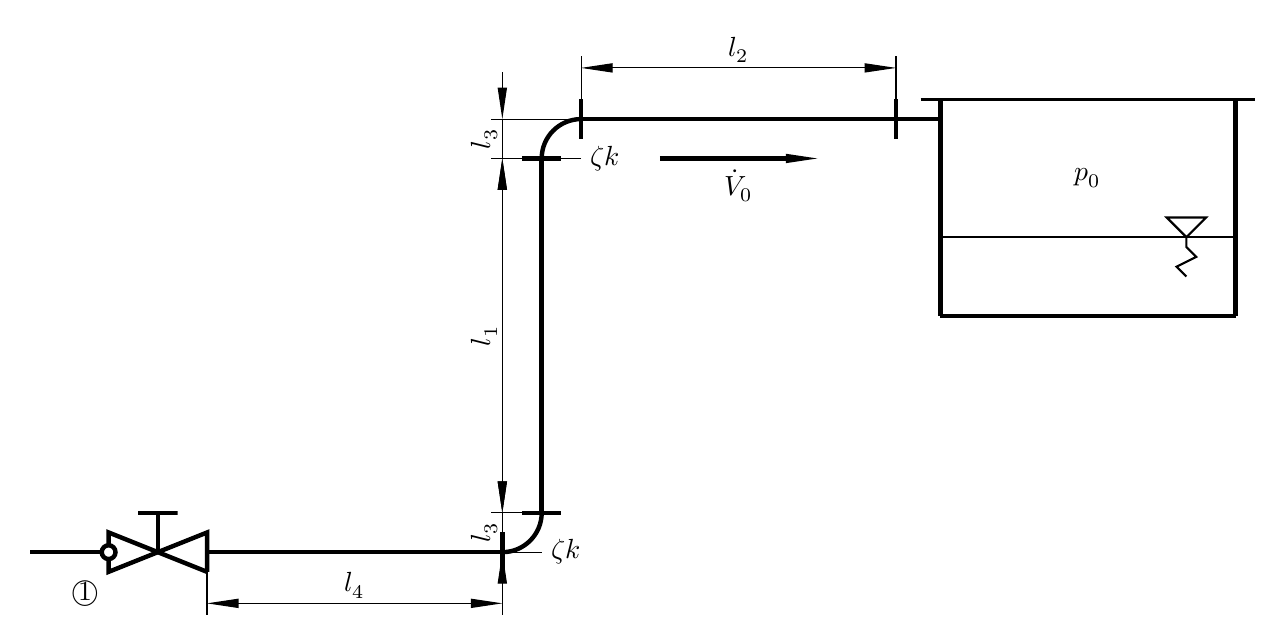
\begin{tikzpicture}
		
	% Változók
	
	\pgfmathsetmacro{\zoom}{2.5}		   	%scaleli a rajzot
	\pgfmathsetmacro{\Legy}{2*\zoom}	 %L1 hosszméret
	\pgfmathsetmacro{\Lketto}{2*\zoom}	 %L2 hosszméret
	\pgfmathsetmacro{\Lharom}{0.2*\zoom} %L3 hosszméret
	\pgfmathsetmacro{\Lnegy}{1.5*\zoom}	 %L4 hosszméret
	\pgfmathsetmacro{\Thossz}{1.5*\zoom}	 %Tartály hossza
	\pgfmathsetmacro{\Tmag}{1*\zoom}		 %Tartály magassága
	\pgfmathsetmacro{\Csat}{0.1*\zoom}	 %Csatlakozóperem, tartályperem, kukacvonal méret
	\pgfmathsetmacro{\Kukac}{0.05*\zoom}
	
	\pgfmathsetmacro{\Tnullx}{\Lharom+\Lketto+0.025*\zoom}
	\pgfmathsetmacro{\Tnully}{\Legy+\Lharom}
	\pgfmathsetmacro{\Vizsz}{1}	%vízszint
	\pgfmathsetmacro{\Trix}{1.25*\zoom}	%kis háromszög helye a vízfelszínen
	\pgfmathsetmacro{\Vszel}{0.5*\zoom} %szelep hossza
	\pgfmathsetmacro{\Vmag}{0.1*\zoom} %szelep magassága
	\pgfmathsetmacro{\Vkor}{0.035*\zoom} %szelepbogyóméret
	\pgfmathsetmacro{\Vekt}{0.4*\zoom}
	
	% Csövek idomok és csőperemek (0,0 az alsó könyök bal oldalánál)
	\draw[ultra thick] 	(-\Lnegy,0)--(0,0); 																	%l4 vonal
	\draw[ultra thick] (0,-\Csat)--(0,\Csat);																	%első könyök előtti perem
	\draw[ultra thick] (0, 0) arc [radius=\Lharom, start angle=270, end angle=360];								%első könyök
	\draw[ultra thick] 	(\Lharom-\Csat,\Lharom)--(\Lharom+\Csat,\Lharom);										%első könyök utáni perem
	\draw[ultra thick] 	(\Lharom,\Lharom)--(\Lharom,\Legy);														%l1 vonal
	\draw[ultra thick] 	(\Lharom-\Csat,\Legy)--(\Lharom+\Csat,\Legy);											%második könyök előtti perem
	\draw[ultra thick] (\Lharom,\Legy) arc [radius=\Lharom, start angle=180, end angle=90];						%második könyök
	\draw[ultra thick] (2*\Lharom, \Legy+\Lharom+\Csat)--(2*\Lharom,\Legy+\Lharom-\Csat);						%második könyök utáni perem
	\draw[ultra thick] (2*\Lharom, \Legy+\Lharom)--(\Lketto,\Legy+\Lharom);										%l2 vonal
	\draw[ultra thick] (\Lketto,\Lharom+\Legy-\Csat)--(\Lketto,\Lharom+\Legy+\Csat); 							%tartály előtti perem
	\draw[ultra thick] (\Lketto,\Legy+\Lharom)--(\Tnullx,\Tnully);												%tartály betöltő csonk
	
	% Tartály
	\draw[ultra thick] (\Tnullx,\Tnully+\Csat)--(\Tnullx,\Tnully-\Tmag);										%tartály ball oldal
	\draw[ultra thick] (\Tnullx,\Tnully-\Tmag)--(\Tnullx+\Thossz,\Tnully-\Tmag);								%tartály alja
	\draw[ultra thick] (\Tnullx+\Thossz,\Tnully-\Tmag)--(\Tnullx+\Thossz,\Tnully+\Csat);						%tartály jobb oldala		
	\draw[thick] (\Tnullx-\Csat,\Tnully+\Csat)--(\Tnullx+\Thossz+\Csat,\Tnully+\Csat);							%tartály fedele
	\draw[thick] (\Tnullx,\Tnully-\Tmag+\Vizsz)--(\Tnullx+\Thossz,\Tnully-\Tmag+\Vizsz);						%vízfelszín
	\draw[thick] (\Tnullx+\Trix,\Tnully-\Tmag+\Vizsz) -- 
		(\Tnullx+\Trix-\Csat,\Tnully-\Tmag+\Vizsz+\Csat)--		
		(\Tnullx+\Trix+\Csat,\Tnully-\Tmag+\Vizsz+\Csat)--
		(\Tnullx+\Trix,\Tnully-\Tmag+\Vizsz);						%kis háromszög	
	
	\draw[thick](\Tnullx+\Trix,\Tnully-\Tmag+\Vizsz)--
		(\Tnullx+\Trix,\Tnully-\Tmag+\Vizsz-\Kukac)--
		(\Tnullx+\Trix+\Kukac,\Tnully-\Tmag+\Vizsz-2*\Kukac)--
		(\Tnullx+\Trix-\Kukac,\Tnully-\Tmag+\Vizsz-3*\Kukac)--
		(\Tnullx+\Trix,\Tnully-\Tmag+\Vizsz-4*\Kukac);		%kukacvonal
	
	% Csap
	\draw[ultra thick] (-\Lnegy,-\Vmag)--
		(-\Lnegy,\Vmag)--
		(-\Lnegy-\Vszel,-\Vmag)--
		(-\Lnegy-\Vszel,0-\Vkor);	
			
	\draw[ultra thick] (-\Lnegy-\Vszel,0) circle (\Vkor);
	\draw[ultra thick] (-\Lnegy-\Vszel,0+\Vkor)--
		(-\Lnegy-\Vszel,\Vmag)--
		(-\Lnegy,-\Vmag);	%test
		
	\draw[ultra thick] (-\Lnegy-\Vszel/2,0)--
		(-\Lnegy-\Vszel/2,2*\Vmag)--
		(-\Lnegy-\Vszel/2+\Csat,2*\Vmag)--
		(-\Lnegy-\Vszel/2-\Csat,2*\Vmag);	%szelep
		
	\draw[ultra thick] (-\Lnegy-\Vszel-\Vkor,0)--(-\Lnegy-\Vszel-1,0);	%bejövő ág
	
	%Méretek
	\pgflength[ xa={-\Lnegy}, ya={-0}, xb={0}, yb={0},ra={0.65} ]{$l_{4}$};				%l4			
	\pgflength[ xa={\Lharom}, ya={0}, xb={\Lharom}, yb={\Lharom},ra={-\Lharom} ]{$l_{3}$};		%l3 alsó	
	\pgflength[ xa={\Lharom}, ya={\Lharom}, xb={\Lharom}, yb={\Legy},ra={-\Lharom} ]{$l_{1}$};		%l1
	\pgflength[ xa={2*\Lharom}, ya={\Legy}, xb={2*\Lharom}, yb={\Lharom+\Legy},ra={-2*\Lharom} ]{$l_{3}$}	%l3 felső	
	\pgflength[ xa={2*\Lharom}, ya={\Lharom+\Legy}, xb={\Lketto}, yb={\Lharom+\Legy},ra={-0.65} ]{$l_{2}$};		%l2	
	
	%Felíratok
	\node[anchor=west] at (\Lharom, 0) {$\zeta{k}$};	 %also kszi
	\node[anchor=west] at (2*\Lharom, \Legy) {$\zeta{k}$};	 %felső kszi
	\node[anchor=north] at (\Tnullx+\Thossz/2, \Legy) {$p_{0}$};	 %p0	
	\node[anchor=north east] at (-\Lnegy-\Vszel,-\Vmag) {\textcircled{1}};	 %1
	\draw[->, ultra thick] (\Lharom-\Vekt+\Lketto/2,\Legy) -- (\Lharom+\Vekt+\Lketto/2,\Legy)
	node[midway, anchor=north,]{$\dot{V}_0$};	%térfogatáram iránya
	
	\end{tikzpicture}
	\caption{Vezetékrendszer}
\end{figure}

\noindent A feladat megoldásához először fel kell venni egy áramvonalat amire fel tudjuk írni a veszteséges Bernoulli egyenletet. Mivel az 1-es pont nyomását keressük, célszerűen az lesz az áramvonal egyik végpontja, a másik végpont a tartály betöltő csonkjánál lesz, ahol ismerjük a nyomást.

\begin{equation}
\dfrac{v_{1}^{2}}{2} + \dfrac{p_{1}}{\varrho} +  gz_{1}
=
\dfrac{v_{2}^{2}}{2} + \dfrac{p_{2}}{\varrho} +  gz_{2} + Y_{vesz}
\end{equation}

\noindent Végezzük el a megfelelő egyszerűsítéseket. Az áramlási sebességet tartalmazó tagok egyenlőek, így kiesnek. Az egyes pont magasságát vegyük $z_{1} = \SI{0}{\m}$-nek. 

\begin{equation}
 \dfrac{p_{1}}{\varrho}
=
 \dfrac{p_{2}}{\varrho} +  gz_{2} + Y_{vesz}
\end{equation}

\noindent A $\varrho$ sűrűséggel átszorozva az egyenletet $p_{1}$ nyomásra rendeztük. Ezzel együtt bontsuk fel a $z_{2}$ értékét.

\begin{equation}
{p_{1}} = {p_{2}} + g (l_{1}+2 \cdot l_{3}) {\varrho} + Y_{vesz} {\varrho}
\end{equation}

\noindent A következő lépés az $Y_{vesz}$ veszteségi tag kifejezése.

\begin{equation}
Y_{vesz} = \zeta \dfrac {v_{atl}^2}{2} =\lambda \dfrac{l_{egyen}}{d} \dfrac {v_{atl}^2}{2}
\end{equation}

\noindent Látható, hogy két ismeretlen tagunk is van, az egyik az $l_{egyen}$ egyenértékű csőhossz a másik pedig a $v_{atl}$ áramlási sebesség, ezeket kell kifejeznünk.

\begin{equation}
l_{egyen} = l_{1}+l_{2}+2l_{3}+l_{4}+\dfrac{d}{\lambda}(\zeta_{T}+2\zeta_{k}+1)
\end{equation}

\begin{equation}
l_{egyen} = \SI{2}{\m}+\SI{2}{\m}+2 \cdot \SI{0,1}{\m}+\SI{30}{\m}+\dfrac{\SI{0,05}{\meter}}{0,025}(0,8+2\cdot 0,15 +1)=\SI{38,4}{\meter}
\end{equation}

\begin{equation}
\dot{V} = v \cdot A 
v=\dfrac{\dot{V}}{A} =\dfrac{\dot{V}}{\dfrac{d^2\pi}{4}} =
	\dfrac{4\dot{V}}{d^2\pi}=
	\dfrac{4\cdot 3 \cdot 10^{-3} \si{\meter\cubed\per\second}}{0,05^2\si{\m\squared}\pi}=
	\dfrac{12\cdot 10^{-3} \si{\meter\cubed\per\second}}{2,5\cdot 10^{-3}\si{\m\squared}\pi}=
	\SI{1,53}{\meter\per\second}
\end{equation}

\noindent A kiszámított értékeket helyettesítsük vissza a $Y_{vesz}$ egyenletébe.

\begin{equation}
Y_{vesz} =\lambda \dfrac{l_{egyen}}{d} \dfrac {v_{atl}^2}{2} =
 0,025 \dfrac{\SI{38,4}{\meter}}{\SI{0,05}{\meter}} \dfrac {1,53^2\si{\meter\squared\per\second\squared}}{2}=
 \SI {22,47}{\joule\per\kilogram}
\end{equation}

\noindent A veszteségi tényezőt az egyszerűsített Bernoulli egyenletbe behelyettesítve meghatározható az egyes pontban a nyomás.

\begin{equation}
{p_{1}} = {p_{2}} + g (l_{1}+2 \cdot l_{3}) {\varrho} + Y_{vesz} {\varrho} = {10^5}\si{\pascal} + \SI {9,81}{\meter\per\second\squared} (\SI{2}{\m} + 2 \cdot \SI{0,1}{\m}) 10^3 \si{\kg\per\meter\cubed} + \SI {22,47}{\joule\per\kilogram} 10^3 \si{\kg\per\meter\cubed}
\end{equation}

\noindent A végeredmény :
\begin{equation}
{p_{1}} = {144052}\si{\pascal}
\end{equation}

% 4/10 Szívócső számítása


% 4/11 Csővezeték méretezése


\chapter{Összenyomhatatlan folyadék egyméretű áramlása}

% 5/1 Pitot--Prandtl-cső


% 5/2 Billenőgyűrűs manométer


% 5/3 Venturi-mérő veszteséges számítása


% 5/4


% 5/5


% 5/6


% 5/7



\end{document}